
\centerline{\textbf{ \LARGE  Properties Regular Languages }}

\begin{enumerate}
    \item properties \\
        \begin{myTableStyle} \begin{tabular}{ |m{14cm}| } \hline
               \begin{center} 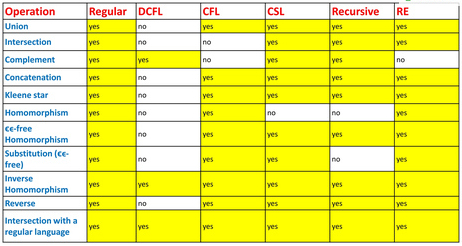
\includegraphics[scale=3.5]{./images/properties.jpeg}  \end{center}\\\hline
        \end{tabular}\end{myTableStyle} \vspace{0.08in}
    \item Every subset of a regular set is regular. [F]
    \item Every finite set is regular. [T]
    \item Union of two non regular sets is not regular. [F]
    \item Infinite union of finite sets is regular. [F]
    \item Let there be 2 languages L1, L2, such that L1 = {\large \( \phi \)}. Then L1.L2 = {\large \(\phi\) } [T]
    \item Regular language is closed under - Union, Intersection, Kleene Closure, Concatenation, Complementation, Difference, Reversal
    \item Context free languages are closed under - Union, Concatenation and Kleene closure
    \item Context free languages are not closed under - Intersection and Complement.
    \item Properties for intersection and difference are same.

\end{enumerate}



\begin{comment}

    \( \mathbf {  } \)  \text{a}^\text{b}  \text{a}^*

    (00)^*   \lambda   \phi

\end{comment}
